\section{Use of HCAL in Classification}\label{app:classification_HCAL}

Since the GoogLeNet architecture was quite large and required significant memory usage and computational power, we decided to investigate the possibility of leaving out HCAL cell-level information, since most of the particle shower occurs in the ECAL. Using our best-performing DNN architecture, we ran ten training sessions with HCAL information, and ten training sessions without HCAL. Averaged training curves from these runs are shown in Figures~\ref{fig:HCAL_study_elechpi} and~\ref{fig:HCAL_study_gammapi0}. These studies demonstrated that including the HCAL caused little to no improvement in classification accuracy. For memory purposes, we thus kept HCAL cell-level information out of our GN architecture. Summed HCAL energy was still fed as an input to the combined classification-regression net, for use in energy regression.

\begin{figure}[htbp]
\centering
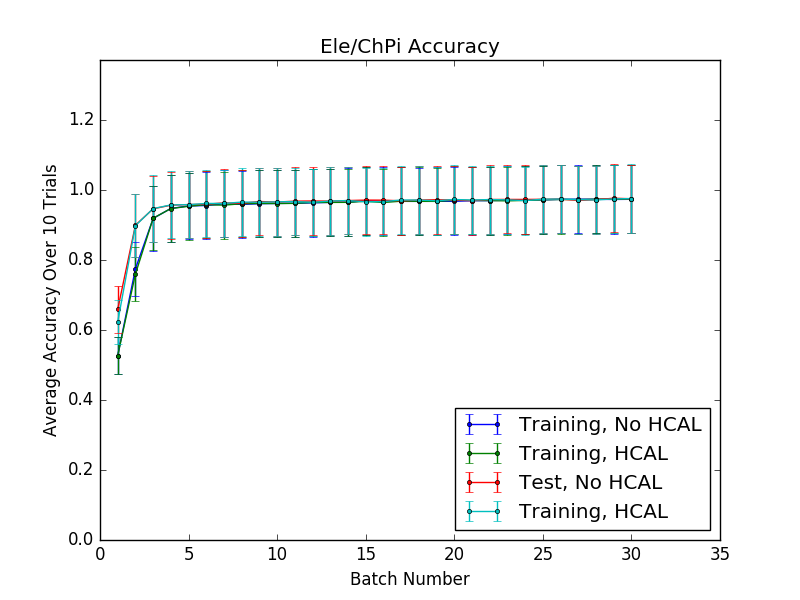
\includegraphics[width=0.38\textwidth]{images/HCAL_study_elechpi_accuracy.png}
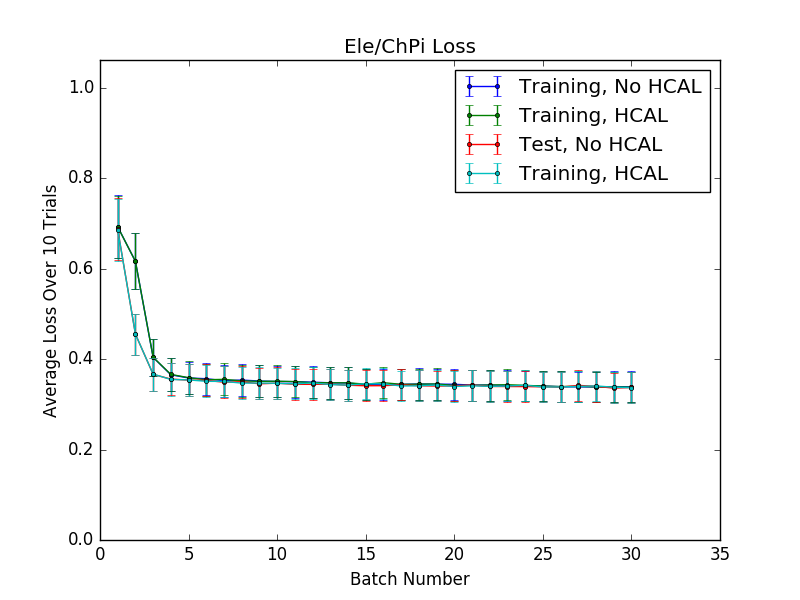
\includegraphics[width=0.38\textwidth]{images/HCAL_study_elechpi_loss.png}
\caption{Accuracy and loss curves for electron/charged pion classification, with and without HCAL cells, using best DNN architecture.}
\label{fig:HCAL_study_elechpi}
\end{figure}

\begin{figure}[htbp]
\centering
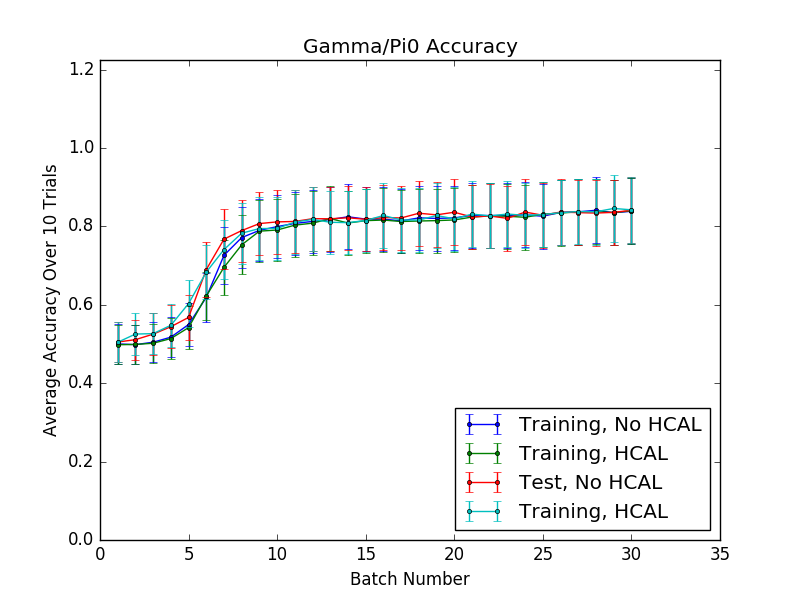
\includegraphics[width=0.38\textwidth]{images/HCAL_study_gammapi0_accuracy.png}
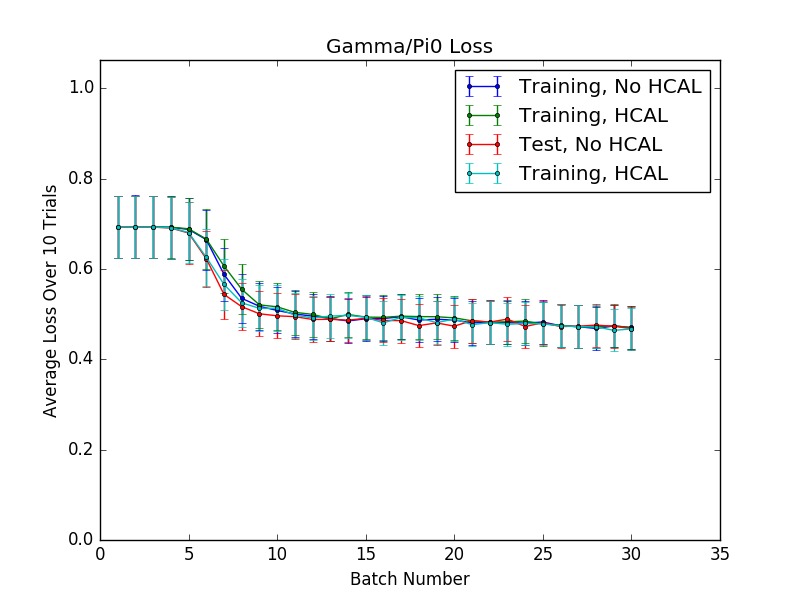
\includegraphics[width=0.38\textwidth]{images/HCAL_study_gammapi0_loss.png}
\caption{Accuracy and loss curves for photon/neutral pion classification, with and without HCAL cells, using best DNN architecture.}
\label{fig:HCAL_study_gammapi0}
\end{figure}